\documentclass[20pt,margin=1in,innermargin=-4.5in,blockverticalspace=-0.3in]{tikzposter}
\geometry{paperwidth=42in,paperheight=30in}
\usepackage[utf8]{inputenc}
\usepackage{amsmath}
\usepackage{amsfonts}
\usepackage{amsthm}
\usepackage{amssymb}
\usepackage{mathrsfs}
\usepackage{graphicx}
\usepackage{adjustbox}
\usepackage{enumitem}
\usepackage{booktabs}
\usepackage{array}
\usepackage{caption}
\usepackage[backend=biber,style=numeric,sorting=none]{biblatex}
\usepackage{emory-theme}

\usepackage{mwe} % for placeholder images

\addbibresource{refs.bib}
\renewcommand*{\bibfont}{\fontsize{17}{12}\selectfont}

% set theme parameters
\tikzposterlatexaffectionproofoff
\usetheme{EmoryTheme}
\usecolorstyle{EmoryStyle}

\title{Bias-Correcting Daily Satellite-Retrieved AOD For Air Quality Research}
\author{Wyatt G.\relax ~Madden\textsuperscript{$\dagger$}, Yang\relax ~Liu\textsuperscript{$\ddagger$}, Howard H.\relax ~Chang\textsuperscript{$\dagger$}}
\institute{\textsuperscript{$\dagger$}Department of Biostatistics \& Bioinformatics, Emory University,\\
\textsuperscript{$\ddagger$}Department of Environmental Health, Emory University\\}
%\titlegraphic{
\includegraphics[width=0.07\textwidth]{wgm_qr.png}}
%\titlegraphic{
\includegraphics[width=0.07\textwidth]{Emory_vt_280.png}}

% begin document
\begin{document}
\maketitle
\centering
\begin{columns}
    \column{0.25}
    \block{Introduction}{
        Fine particulate matter ($PM_{2.5}$) is a major air pollutant that is associated with adverse health outcomes.
        Typically $PM_{2.5}$ is measured at ground level monitoring stations, however these stations are globally sparse and provide poor coverage for many areas that experience high air pollution levels. 
        The National Aeronautics and Space Administration (NASA) selected the Multi Angle Imager for Aerosols (MAIA) proposal in 2016 to improve this coverage and better understand how respirable particulate matter ($PM_{2.5}$) affects human health.\cite{liu2017}
        The MAIA project will deploy satellites to collect global 1-km spatial resolution Aerosol Optical Depth (AOD) data. 
        AOD strongly correlates with $PM_{2.5}$, and thus can be used to better understand adverse health outcomes by employing bias-correcting methods. 

    \vspace{1em}
    \begin{tikzfigure}[PM2.5 observations on 2018-10-08 at all AQI monitors in the contiguous United States.]
        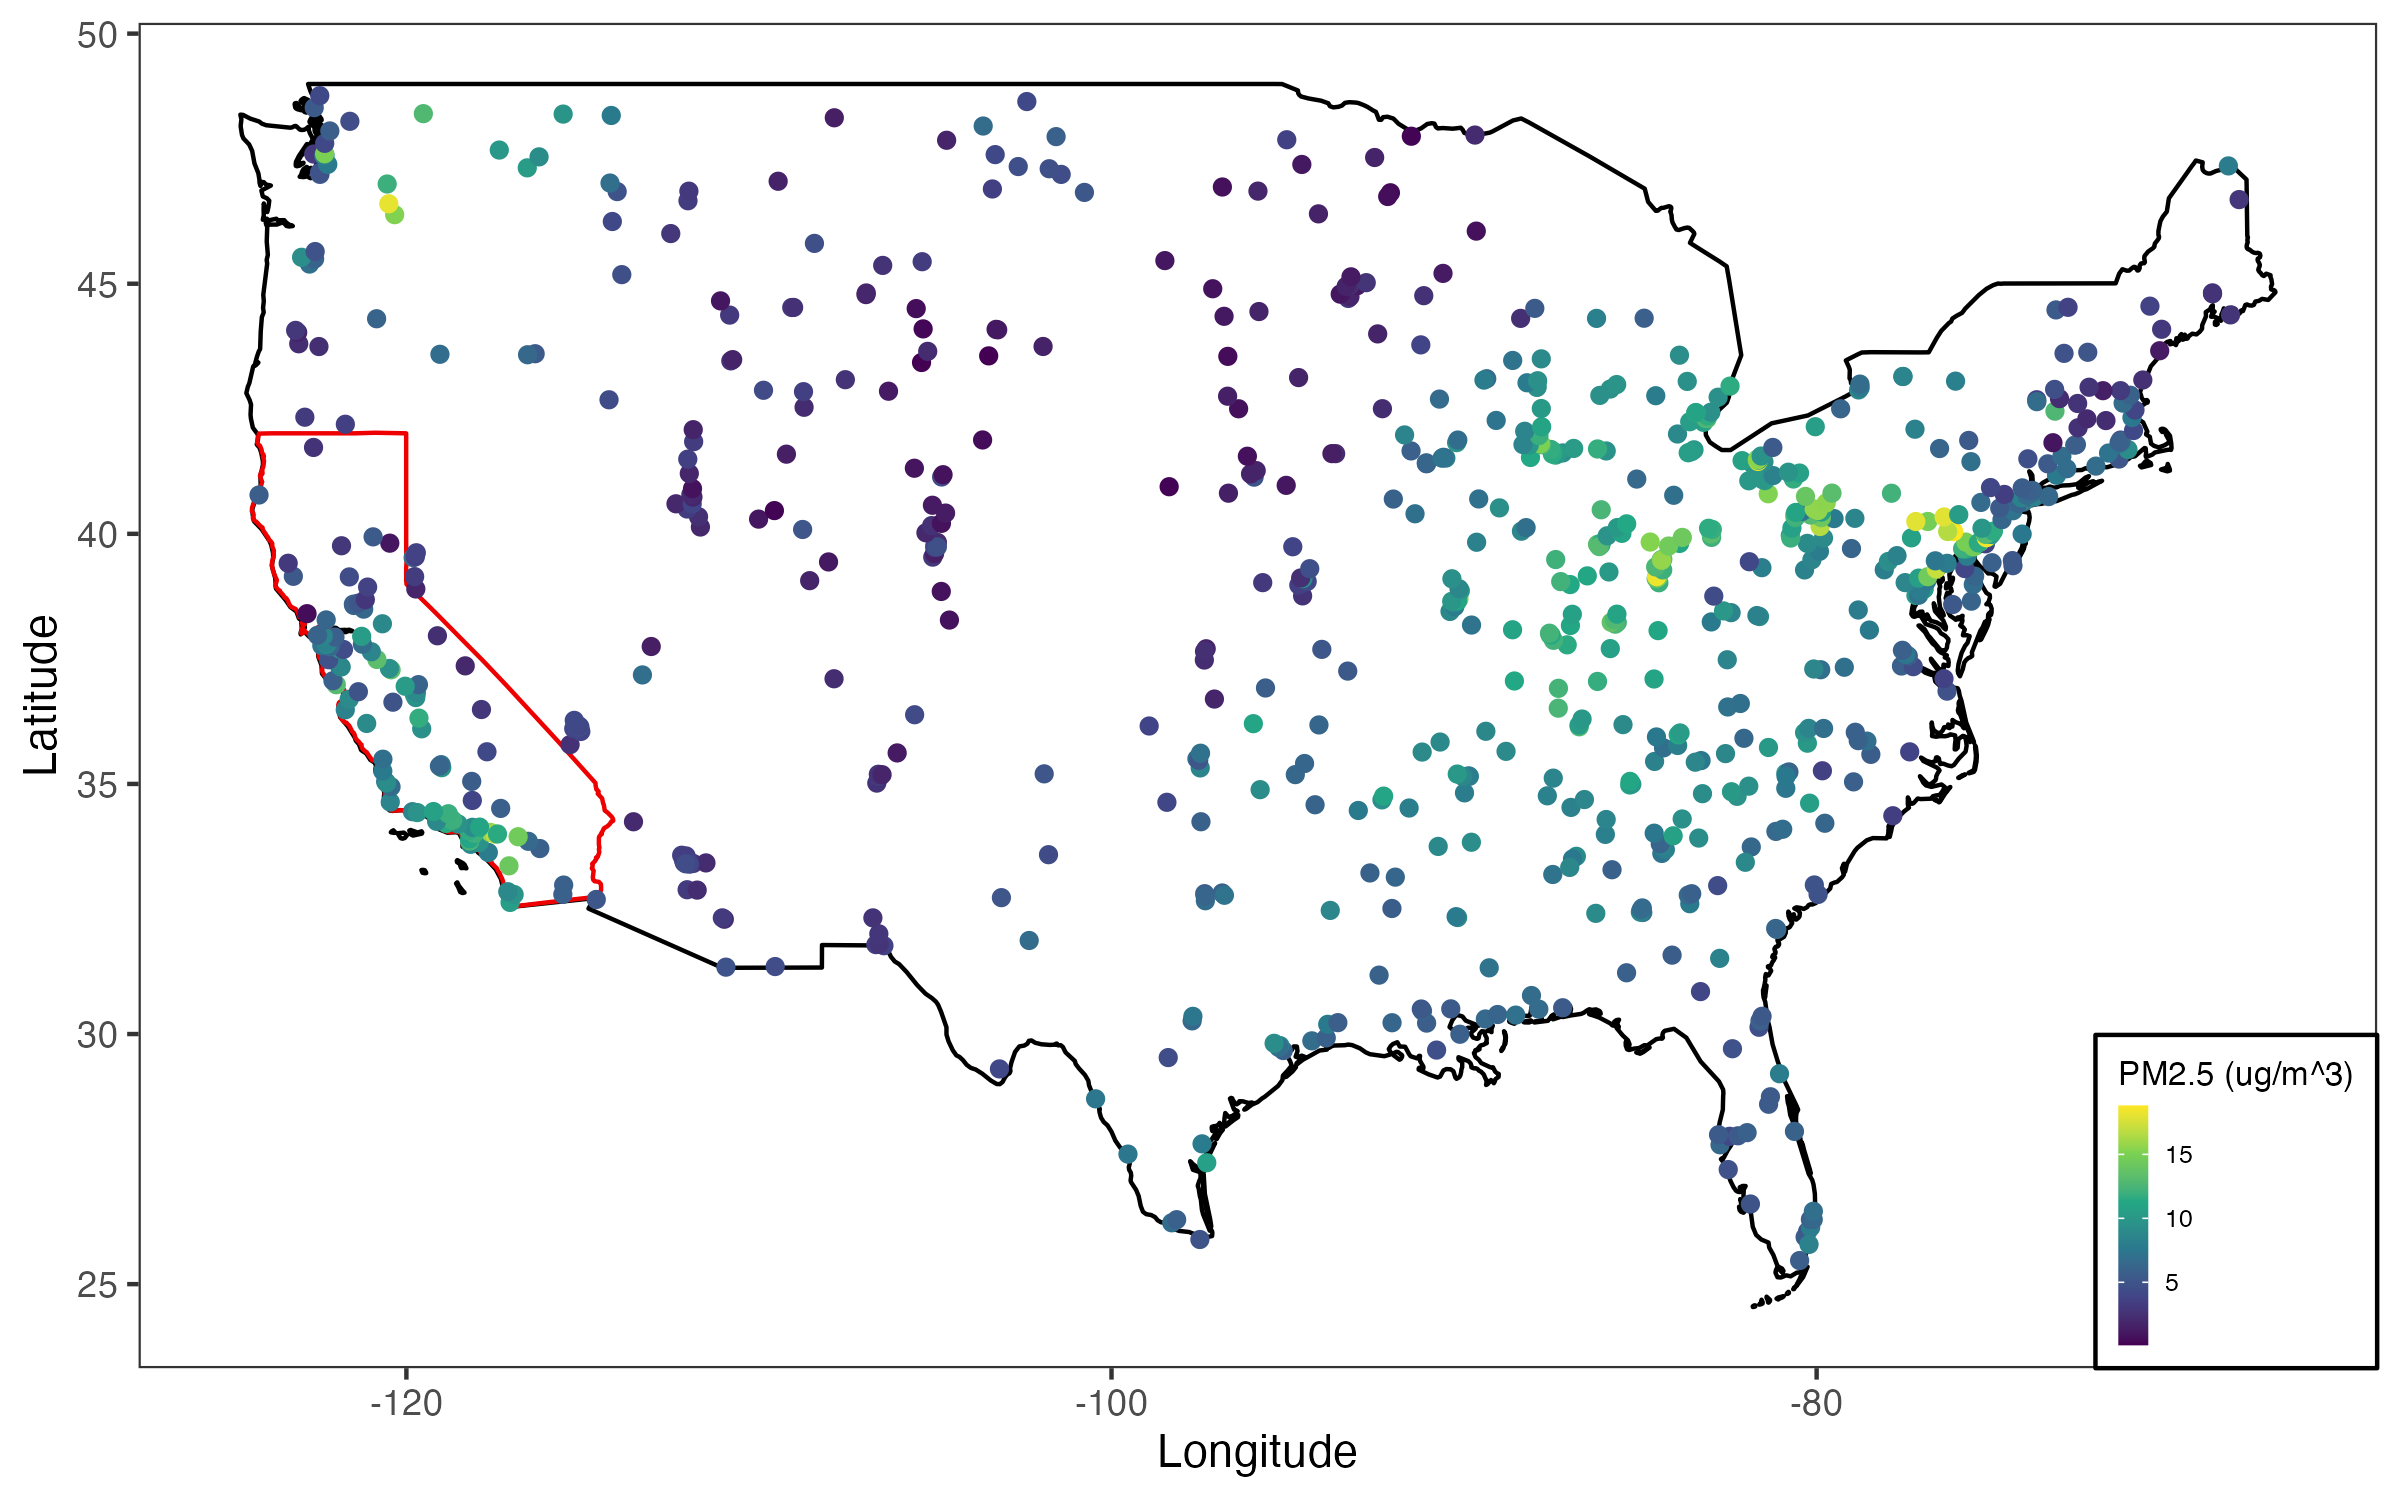
\includegraphics[width=0.7\linewidth]{figures/obs_map_20181008.png}
        \label{fig:obs_map}
    \end{tikzfigure}
    \vspace{1em}

        While bias-correcting satellite or numerical model simulations with ground-level monitoring data is a common task in air quality modeling, Bayesian uncertainty quantification is not widely adopted in part due to lack of user-friendly implementations. 

        Here we present a Bayesian geostatistical regression model framework and corresponding R package (\texttt{grmbayes}) to efficiently estimate the relationship between satellite/simulation air quality data and ground monitor collected $PM_{2.5}$, and predict $PM_{2.5}$ at locations for which only satellite/simulation data is available. 
        This software will provide scientists and practitioners with a user-friendly tool to employ Bayesian spatio-temporal methods when incorporating MAIA data in air quality research.
        \vspace{1em}
        \begin{tikzfigure}[Histogram of PM2.5 observations across all AQI monitors and days in 2018.]
            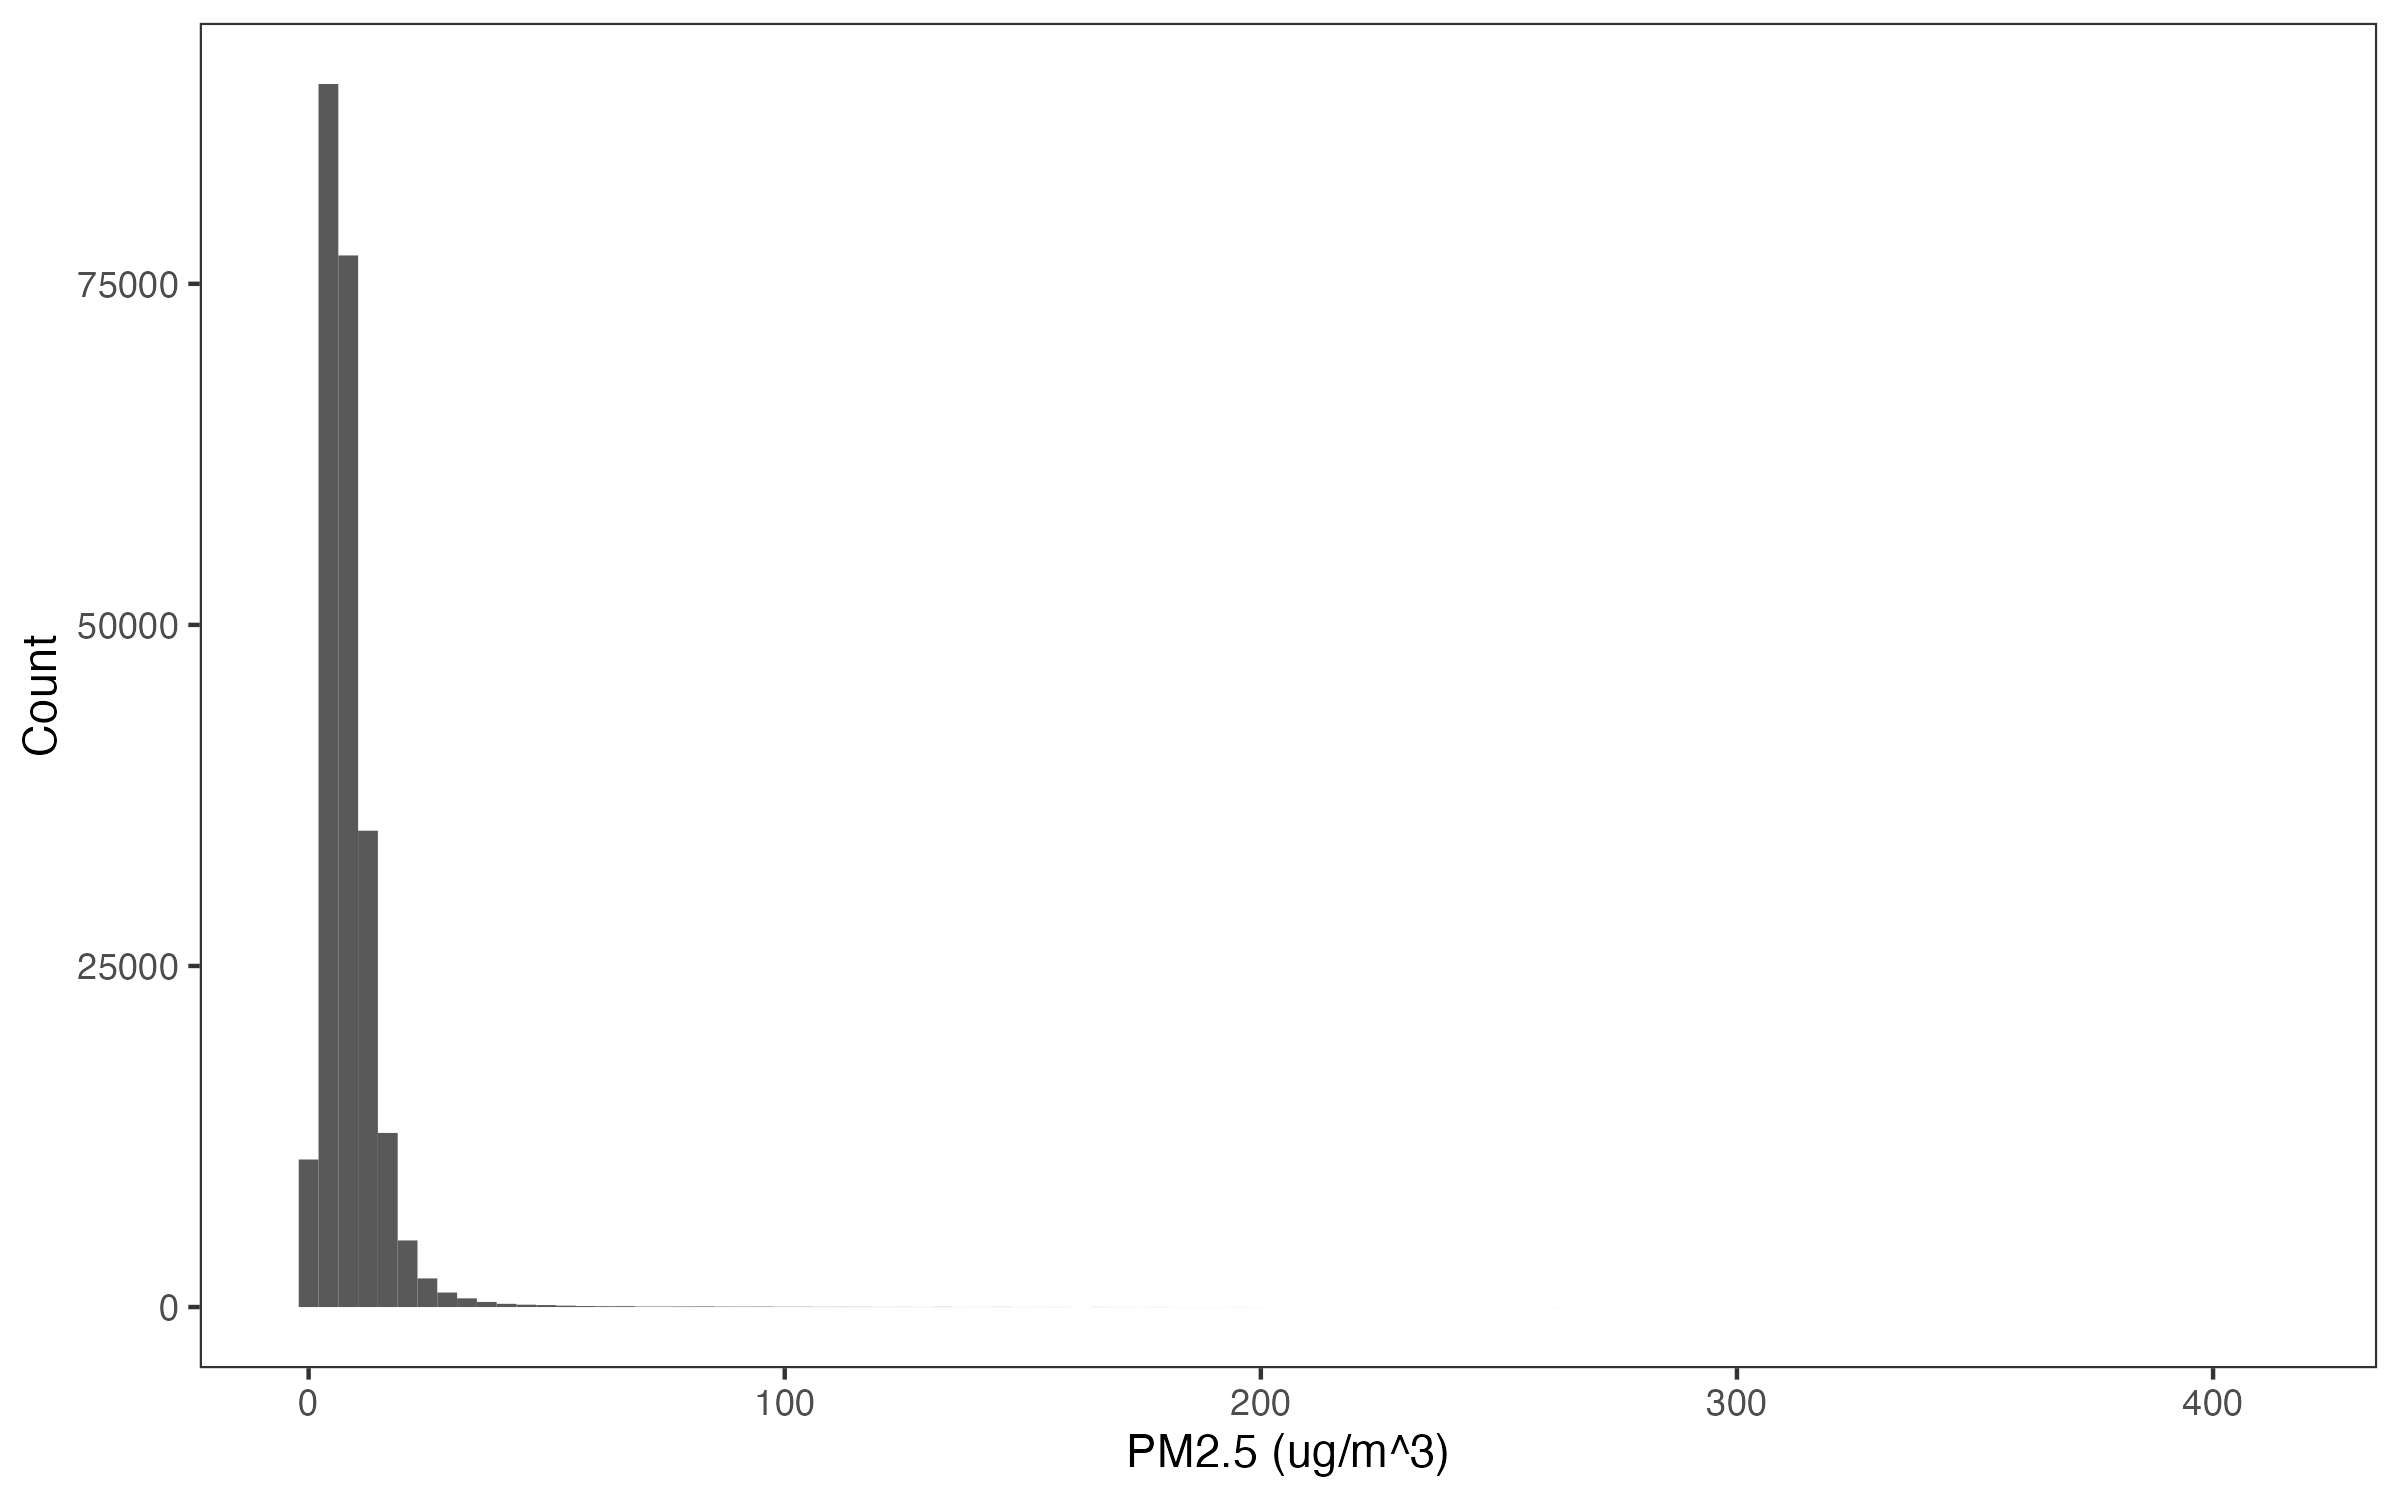
\includegraphics[width=0.7\linewidth]{figures/histogram_all.png}
        \label{fig:histogram}
        \end{tikzfigure}
        \vspace{1em}
    }
    \column{0.25}
    \block{Data}{


    Our data consists of daily $PM_{2.5}$ observations from 2018 at 973 ground-level air quality monitors in the contiguous United States.\relax(Figure~\ref{fig:obs_map})
    These data were chosen due to the large number of major wildfire events, most notably the Camp Fire in California, which corresponded with high $PM_{2.5}$ variability.\relax(Table~\ref{tab:monthly_stat}, Figure~\ref{fig:histogram})
    While our motivation and exposition assumes regressing on MAIA AOD data, we utilize 12km gridded Community Multiscale Air Quality (CMAQ) Chemical Transport Model (CTM) simulation data for our examples throughout this work without loss of generality.\cite{byun2006}
    MAIA AOD data are matched to each monitor by date and location (nearest neighbor) for model fitting while full data sets can be used for $PM_{2.5}$ prediction. 
    

         \begin{center}
             \captionof{table}{Monthly summary statistics of $PM_{2.5}$ observations across all monitors and days.}\label{tab:monthly_stat}

             \resizebox{12cm}{!}{
             
\begin{tabular}{cccccc}
\toprule
Month & Mean & Median & Min & Max & Sd\\
\midrule
Jan & 9.3 & 7.8 & 0.1 & 318.8 & 7.9\\
\\[-3.0ex]
Feb & 8.2 & 6.9 & 0.1 & 71.5 & 5.6\\
\\[-3.0ex]
Mar & 6.6 & 5.8 & 0.1 & 74.0 & 4.2\\
\\[-3.0ex]
Apr & 6.9 & 6.3 & 0.1 & 55.1 & 3.9\\
\\[-3.0ex]
May & 7.6 & 7.1 & 0.1 & 156.0 & 3.9\\
\\[-3.0ex]
Jun & 7.9 & 7.3 & 0.1 & 167.8 & 4.5\\
\\[-3.0ex]
Jul & 9.4 & 8.2 & 0.1 & 146.0 & 6.3\\
\\[-3.0ex]
Aug & 12.4 & 10.1 & 0.1 & 261.0 & 11.0\\
\\[-3.0ex]
Sep & 6.9 & 6.1 & 0.1 & 76.2 & 4.1\\
\\[-3.0ex]
Oct & 6.3 & 5.6 & 0.1 & 43.0 & 3.8\\
\\[-3.0ex]
Nov & 9.7 & 6.7 & 0.1 & 411.7 & 14.2\\
\\[-3.0ex]
Dec & 8.8 & 7.3 & 0.1 & 70.6 & 6.3\\
\bottomrule
\end{tabular}

         }
         \end{center}

    }
    \block{Model}{
         The geostatistical regression model is given by
         \begin{align*} 
             PM_{2.5}(s,t) = \alpha_0(s, t) + \alpha_1(s, t) X(s, t) + \epsilon(s, t)
         \end{align*}
         where $PM_{2.5}(s,t)$ and $X(s, t)$ are the fine particulate matter  concentration and the aerosol optical depth respectively, at location $s$ and time $t$.\cite{chang2014}
    The $\alpha_0(s, t)$ and $\alpha_1(s, t)$ parameters are the intercept and slope of the regression model composed of the following spatial and temporal effects:
    \begin{align*}
        \alpha_0(s, t) = \beta_0(s) + \beta_0(t) + \gamma_0 Z_0 \\
        \alpha_1(s, t) = \beta_1(s) + \beta_1(t) + \gamma_1 Z_1 
    \end{align*} 
    where $\beta_i(s) \sim NNGP(0, \tau_i^2 K_i)$, $\beta_i(t)$ are modeled as first-order random walks, and $\gamma_i$ are fixed effects for spatial or spatio-temporal varying covariates $Z_i$.
    The $K_i$ kernal of the Nearest Neighbor Gaussian Process (NNGP)\cite{datta2014} is assumed Mat\'{e}rn($\nu_i$, $\theta_i$), with $\nu_i \in \{\frac{1}{2}, \frac{3}{2}, \frac{5}{2} \}$, with a pre-specified number of neighbors.
    Weakly-informative priors are placed on all parameters and MCMC is employed to sample from the posterior distribution of the model parameters.
    For computational efficiency, both NNGP and regular GP are assessed in addition to discretization of the spatial process range parameter $\theta_i$. 

    }

    \column{0.25}
    \block{R Package: grmbayes}{
        We provide an intuitive interface for fitting the geostatistical regression model with the following features:
        {
        \fontsize{22pt}{20pt}\selectfont
        \begin{itemize}
            \item \textbf{Spatial Process}: Select either GP or NNGP (with $m$ number of neighbors)
            \item \textbf{Random Effects}: Select either additive or multiplicative random effects for spatial and/or temporal components.
            \item $\pmb{\theta}$ \textbf{Discretization}: Discretize the spatial process range parameter $\theta_i$ for spatial intercept and/or spatial slope. Choose levels, and either Gibbs or Metropolis-Hastings updating schemes. 
            \item \textbf{Cross Validation}: Choose number of folds, and cross validation type (out of `ordinary', `spatial', `spatial clustered' or `spatial buffered' with a corresponding buffer size). 
            \item \textbf{Covariance Kernal}: Select Mat\'{e}rn($\theta$, $\nu$) covariance function with $\nu \in \{\frac{1}{2}, \frac{3}{2}, \frac{5}{2} \}$, or input user-defined covariance kernal.
            \item \textbf{Covariates}: Include additional regression covariates. 
        \end{itemize}
        }
        
    }
    \block{Performance}{

        First we assess the appropriateness of the approximations designed to improve computational efficiency. 
        Setting the number of neighbors to 10 and discretizing the $\theta$ parameters into 20 equally spaced levels across the range of feasible values determined from a non-discretized test run, we fit the models for all combinations of NNGP/GP and discretization schemes for 119 monitors within California.
        All models perform nearly identically \relax (Table~\ref{tab:just_ca_rmse}), suggesting that the approximations are appropriate. 
         \begin{center}
             \captionof{table}{California in-sample RMSE for all combinations of spatial process and $\theta$ discretization schemes.}\label{tab:just_ca_rmse}
             \resizebox{12cm}{!}{
                 
\begin{tabular}{cccc}
\toprule
\multicolumn{1}{c}{ } & \multicolumn{2}{c}{$\theta$ Discretization} \\
\cmidrule(l{3pt}r{3pt}){2-3}
Spatial Process & Gibbs & MH & None\\
\midrule
GP & 8.80 & 8.8 & 8.8\\
NNGP & 8.81 & 8.8 & 8.8\\
\bottomrule
\end{tabular}

         }
         \end{center}
         Next we assess the performance of the model on the full contiguous United States data set for the three settings of Mat\'{e}rn covariance $\nu \in \{\frac{1}{2}, \frac{3}{2}, \frac{5}{2}\}$,  utilizing five 10-fold cross-validation formulations: ordinary, spatial, spatial clustered, and spatial buffered (with buffer size of 35km and 100km).\relax(Table~\ref{tab:full_grid_rmse})
         These results suggest that $\nu = \frac{1}{2}$ (exponential covariance kernal) is most appropriate for these data, and that there is considerable information gained from the spatial components of the model.
         \begin{center}
             \captionof{table}{Full U.S. RMSE (95\% Prediction Interval Coverage Probability) for all combinations of spatial process and $\theta$ discretization schemes.}\label{tab:full_grid_rmse}
             \resizebox{16cm}{!}{
                 
\begin{tabular}{cccc}
\toprule
\multicolumn{1}{c}{ } & \multicolumn{2}{c}{Mat\'{e}rn $\nu$ Parameter} \\
\cmidrule(l{3pt}r{3pt}){2-3}
Cross Validation Type & 0.5 & 1.5 & 2.5\\
\midrule
Ordinary & 5.18 (0.97) & 5.18 (0.97) & 5.18 (0.97)\\
\\[-3.0ex]
Spatial & 5.61 (0.98) & 5.88 (0.98) & 5.9 (0.98)\\
\\[-3.0ex]
Spatial Buffered (35km) & 5.79 (0.98) & 6.03 (0.98) & 6.02 (0.98)\\
\\[-3.0ex]
Spatial Buffered (100km) & 6.12 (0.98) & 6.16 (0.98) & 6.16 (0.98)\\
\\[-3.0ex]
Spatial Clustered & 6.35 (0.98) & 6.43 (0.98) & 6.43 (0.98)\\
\bottomrule
\end{tabular}

         }
         \end{center}
     }


    \column{0.25}

    \block{Prediction}{

        Predictions are made by kriging the nearest neighbor spatial effects from the $PM_{2.5}$ monitor data set for each AOD location, and combining this with temporal effects. \relax (Figures~\ref{fig:preds},~\ref{fig:preds_4})
        
        \vspace{1em}
        \begin{tikzfigure}[PM2.5 mean posterior predictions by season at all prediction locations in the contiguous United States.]
            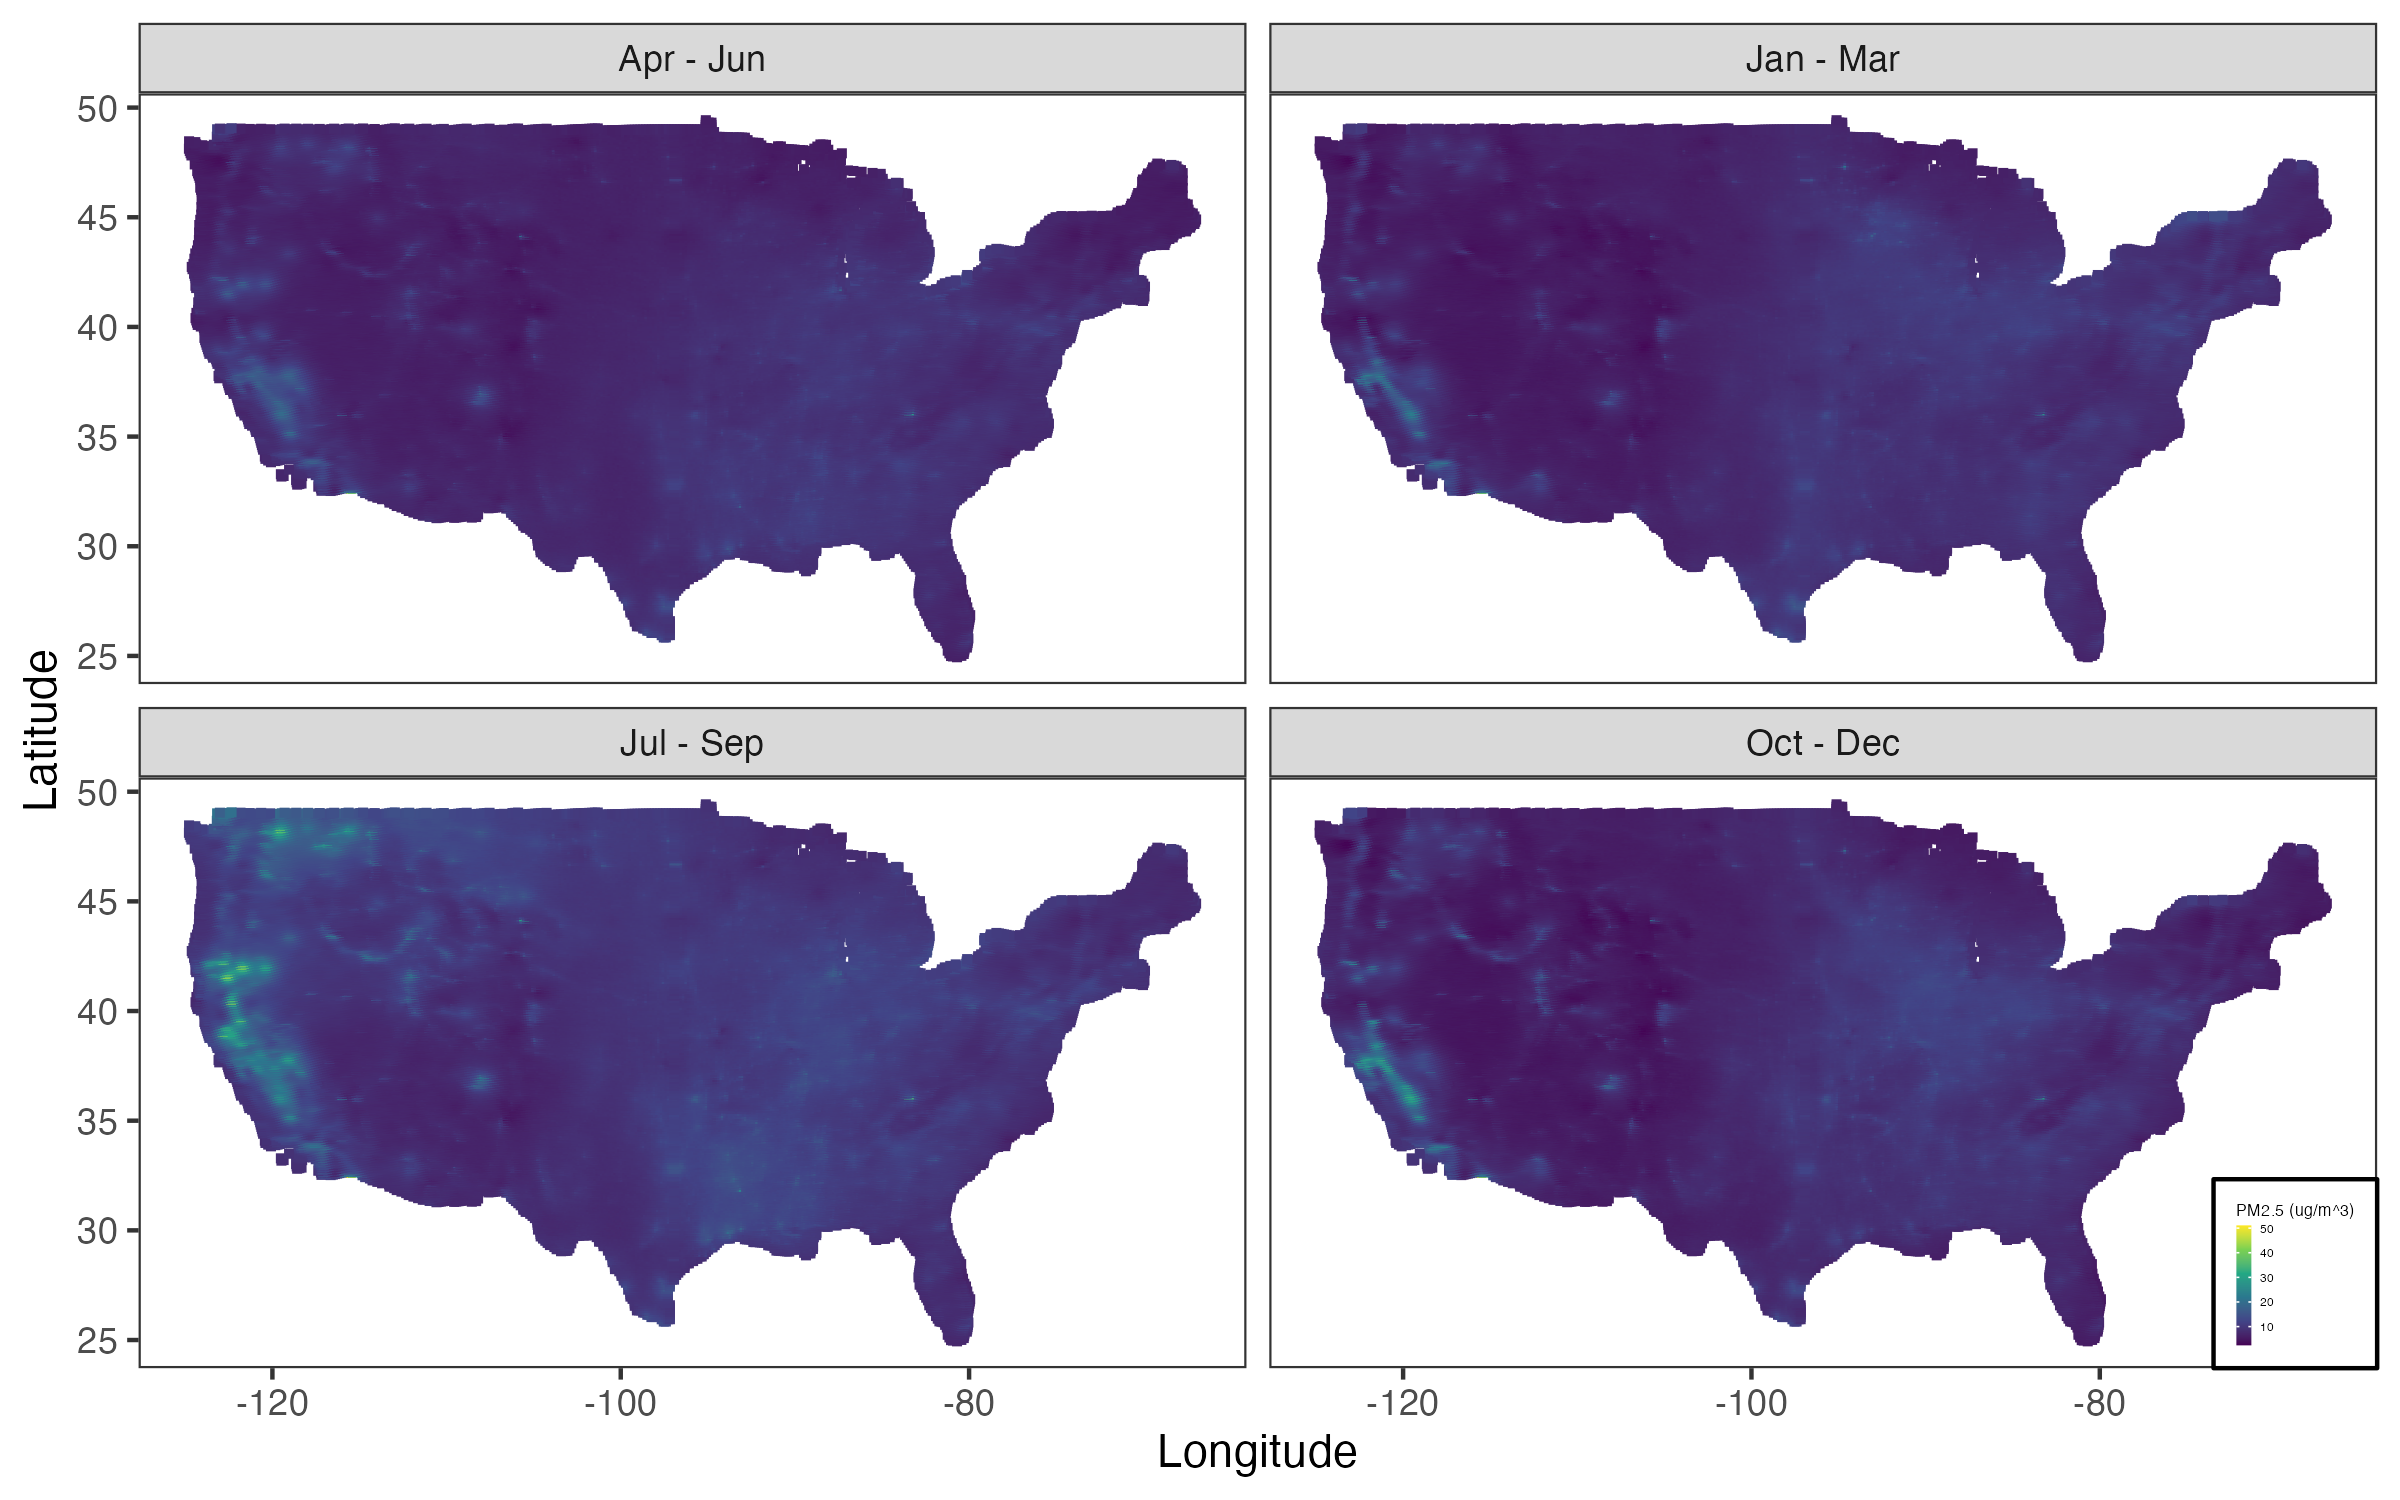
\includegraphics[width=0.7\linewidth]{figures/pred_map_season.png}
             \label{fig:preds_4}
        \end{tikzfigure}
        \begin{tikzfigure}[PM2.5 predictions on 2018-10-08 at all prediction locations in the contiguous United States.]
            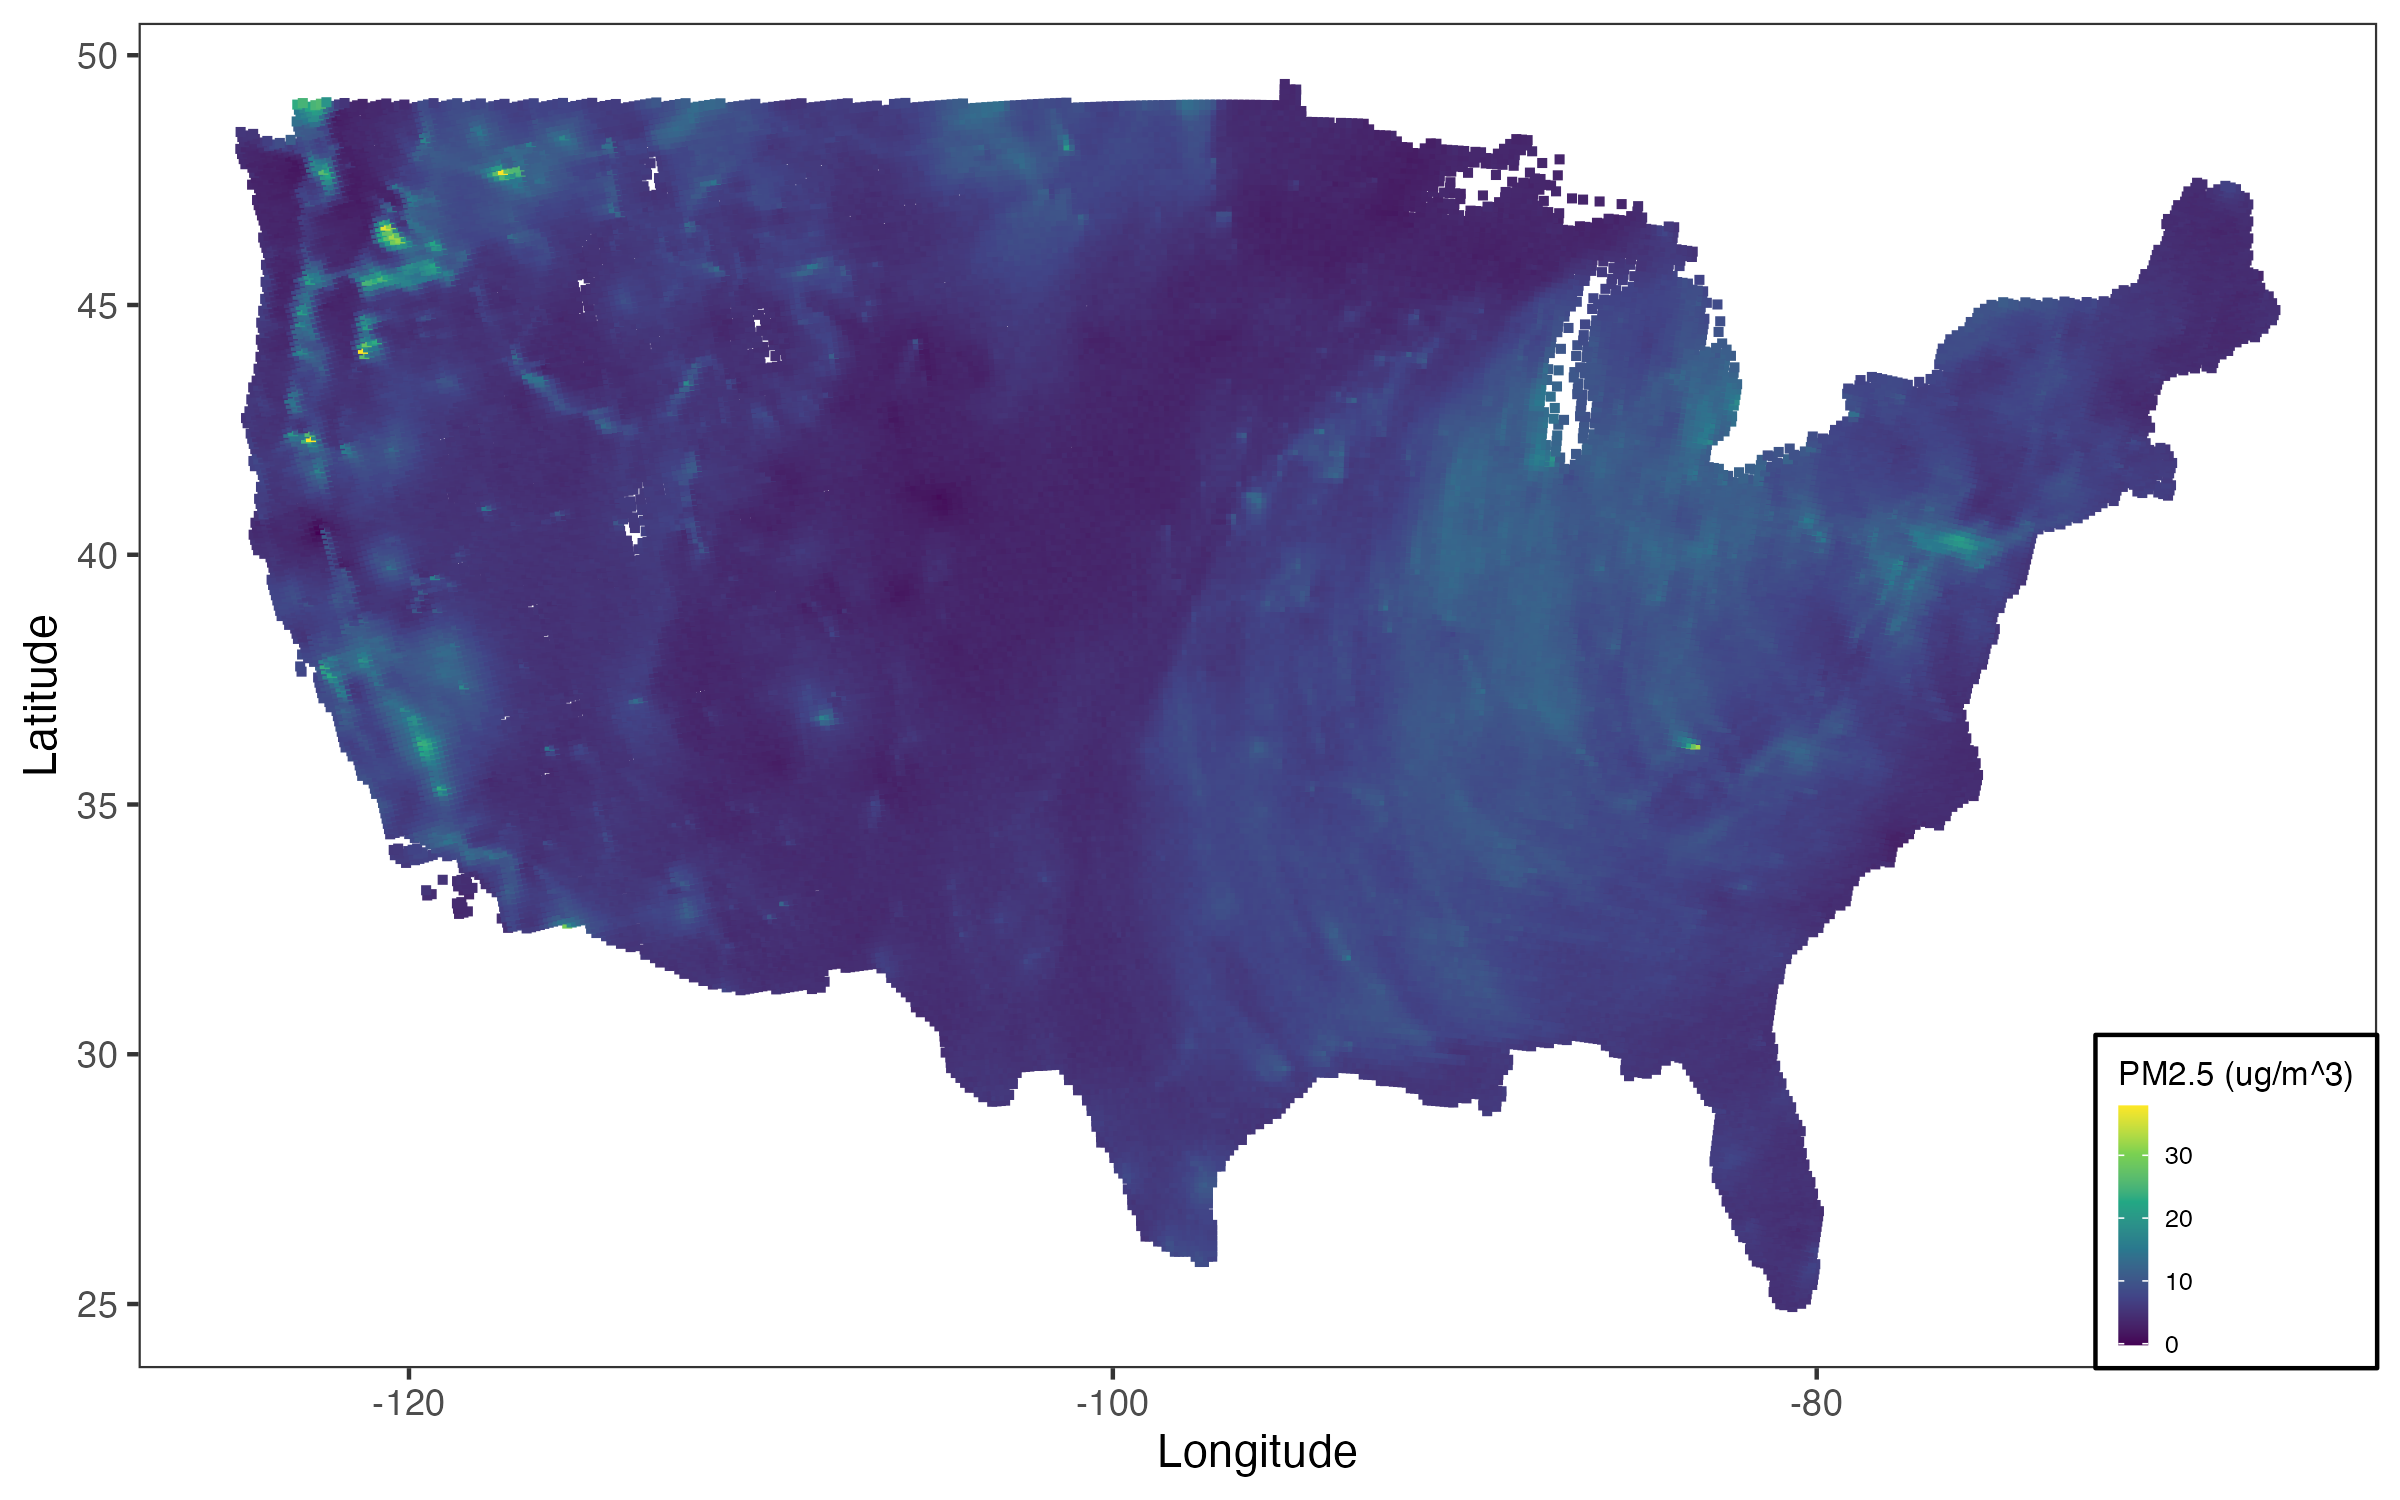
\includegraphics[width=0.7\linewidth]{figures/pred_map_20181008.png}
             \label{fig:preds}
        \end{tikzfigure}


    
    }
    
    \block{Acknowledgements}{
        This project is partially supported by the NASA/JPL EVI-3 Multi-Angle Imager for Aerosols (MAIA) Proposal, and the motivating dataset is provided by Dr. Vaidyanathan at the US CDC Climate and Health Program.\\

    }
    
    \block{References}{
        \vspace{-1em}
        \printbibliography[heading=none]
    }
\end{columns}
\end{document}
